\documentclass[../main/main.tex]{subfiles}

\newdate{date}{06}{11}{2019}


\begin{document}

\marginpar{ \textbf{Lecture 8.} \\  \displaydate{date}. \\ Compiled:  \today.}
\noindent Since \( \sum_{k}^{} \lambda _k^N = Z_N \) for \( k=+,-,1,\dots,n \), we have
\begin{equation*}
  \expval{S_1 S_R}_N = \frac{\sum_{ij}^{} \bra{t_j} \mathbb{S}_1 \ket{t_i} \lambda _i^{R-1} \bra{t_i} \mathbb{S}_R \ket{t_j} \lambda _j^{N-R+1}      }{\sum_{k=1}^{n} \lambda _k^N  }
\end{equation*}
If we now multiply and divide by \( \lambda _+^N \), we get
\begin{equation*}
  \expval{S_1 S_R}_N = \frac{\sum_{ij}^{} \bra{t_j} \mathbb{S}_1 \ket{t_i} (\lambda _i/ \lambda _+)^{R-1}  \bra{t_i} \mathbb{S}_R \ket{t_j} (\lambda _j / \lambda _+)^{N-R+1}    }{\sum_{k=1}^{n} (\lambda _k  / \lambda _+)^{N} }
\end{equation*}
\begin{remark}
In the thermodynamic limit \( N \rightarrow \infty  \), only the terms with \( j=+ \) and \( k=+ \) will survive in the sum. Remind that \( R \) is fixed.
\end{remark}
\begin{equation*}
\expval{S_1 S_R} =   \lim_{N \rightarrow \infty } \expval{S_1 S_R}_N = \sum_{i= \pm,1 \dots n}^{} \qty(\frac{\lambda _i}{\lambda _+})^{R-1} \bra{t_+} \mathbb{S}_1 \ket{t_i} \bra{t_i} \mathbb{S}_R \ket{t_+}
\end{equation*}
Rembember that \( \lambda _+ > \lambda _- \ge \lambda _1 \ge \dots \ge \lambda _n \):
\begin{equation*}
  \expval{S_1 S_R} = \bra{t_+} \mathbb{S}_1 \ket{t_+} \bra{t_+} \mathbb{S}_R \ket{t_+} +   \sum_{i \neq +}^{n} \qty(\frac{\lambda _i}{\lambda _+})^{R-1} \bra{t_+} \mathbb{S}_1 \ket{t_i} \bra{t_i} \mathbb{S}_R \ket{t_+}
\end{equation*}
Since one can prove 
\begin{equation}
  \lim_{N \rightarrow \infty } \expval{S_R}_1 = \bra{t_+} \mathbb{S}_1 \ket{t_+} , \quad \lim_{N \rightarrow \infty } \expval{S_R}_N = \bra{t_+} \mathbb{S}_R \ket{t_+}
  \label{eq:8_3}
\end{equation}
we obtain
\begin{equation}
  \expval{S_1 S_R} = \expval{S_1} \expval{S_R} + \sum_{i \neq +}^{}  \qty(\frac{\lambda _i}{\lambda _+})^{R-1} \bra{t_+} \mathbb{S}_1 \ket{t_i} \bra{t_i} \mathbb{S}_R \ket{t_+}
  \label{eq:8_2}
\end{equation}
\begin{example}{Show relation \eqref{eq:8_3}}{}
Let us prove \eqref{eq:8_3} by a method analogous to that followed above.
\begin{equation*}
\begin{split}
\expval{S_1}_N &= \frac{1}{Z} \sum_{\{ S \} }  S_1 e^{- \beta \mathcal{H}_N}
= \frac{1}{Z} \sum_{S_1} S_1 \bra{S_1}  \mathbb{T}^N \ket{S_1} 
 = \frac{1}{Z} \sum_{S_1} S_1 \sum_{i}  \bra{S_1}\ket{t_i} \lambda_i^N \bra{t_i} \ket{S_1} \\
&= \frac{1}{Z} \sum_{i} \lambda_i^N \bra{t_i} \mathbb{S}_1 \ket{t_i}  
 = \frac{\sum_{i}^{} \qty(\lambda_i/\lambda_+)^N \bra{t_i} \mathbb{S}_1 \ket{t_i}  }{ \sum_{k=1}^{n} (\lambda _k  / \lambda _+)^{N} }
\end{split}
\end{equation*}
Taking the limit \( N \rightarrow \infty \):
\begin{equation*}
\expval{S_1} =   \lim_{N \rightarrow \infty } \expval{S_1}_N = 
\bra{t_+} \mathbb{S}_1 \ket{t_+}
\end{equation*}
\end{example}
The correlation function follows immediately from \eqref{eq:8_2},
\begin{equation}
\Gamma _R =   \expval{S_1 S_R} - \expval{S_1}\expval{S_R} = \sum_{i \neq +}^{n} \qty(\frac{\lambda _i}{\lambda _+})^{R-1} \bra{t_+} \mathbb{S}_1 \ket{t_i} \bra{t_i} \mathbb{S}_R \ket{t_+}
\end{equation}
\begin{remark}
\( \Gamma_R \) depends only on the eigenvalues and eigenvectors of the transfer matrix \( \mathbb{T} \) and by the values of the spins \( S_1 \) and \( S_R \).
\end{remark}
A much simpler formula is obtained for the correlation length \eqref{eq:7_2}. Taking the limit \( R \rightarrow \infty  \) the ratio \( (\lambda _-/ \lambda _+) \) dominates the sum and hence
\begin{equation*}
\begin{split}
\xi ^{-1} &=  \lim_{R \rightarrow \infty } \qty{-\frac{1}{R-1} \log{\qty|\expval{S_1S_R} - \expval{S_1} \expval{S_R}   |} } \\
& = \lim_{R \rightarrow \infty }  \qty{-\frac{1}{R-1} \log{\qty[  \qty(\frac{\lambda _-}{\lambda _+})^{R-1} \bra{t_+} \mathbb{S}_1 \ketbra{t_-}{t_-} \mathbb{S}_R \ket{t_+}  ]  } } \\
& = -\log{\qty[\qty(\frac{\lambda _-}{\lambda _+}) ] } - \lim_{R \rightarrow \infty } \frac{1}{R-1} \log{ \bra{t_+} \mathbb{S}_1 \ketbra{t_-}{t_-} \mathbb{S}_R \ket{t_+}    }  \\
& = - \log{\qty(\frac{\lambda _-}{\lambda _+}) }
\end{split}
\end{equation*}
The important result is
\begin{empheq}[box=\myyellowbox]{equation}
  \xi ^{-1} = -  \log{\qty(\frac{\lambda _-}{\lambda _+}) }
\end{empheq}
It means that the \emph{correlation length does depend only on the ratio between the two largest eigenvalues of the transfer matrix \( \mathbb{T} \)}.


\subsection{Results for the \emph{1-dim} Ising model}
Let us now return to the example of the nearest neighbour Ising model in a magnetic field, to obtain explicit results for the bulk free energy \(f_b\), the correlation function \( \Gamma\) and the correlation length \( \xi \).

Recall that the transfer matrix of such a system is given by
\begin{equation*}
  \mathbb{T} =
  \begin{pmatrix}
  \exp (K+h)     & \exp (-K)  \\
  \exp (-K)    & \exp (K-h)
  \end{pmatrix}
\end{equation*}
Now, let us calculate the eigenvalues:
\begin{equation*}
  \abs{\mathbb{T}-\lambda \mathbb{1}} =  (e^{K+h}- \lambda  )(e^{K-h}-\lambda  )-e^{-2K}=0
\end{equation*}
The two solutions are
\begin{empheq}[box=\myyellowbox]{equation}
  \lambda _{\pm} = e^{K} \cosh(h) \pm \sqrt{e^{2K}\sinh^2 (h)+e^{-2K} }
\end{empheq}
\subsubsection{The free energy}
The free energy is
\begin{equation*}
\begin{split}
    f_b & \equiv \lim_{N \rightarrow \infty } \frac{-k_B T}{N} \log{Z_N (K,h)}   \\
    & = -k_B T \lim_{N \rightarrow \infty } \frac{1}{N}  \log{\qty[\lambda _+^N \qty(1+\qty(\frac{\lambda _-}{\lambda _+})^N ) ] } \\
    & = -k_B T \log{\lambda _+}
\end{split}
\end{equation*}
and inserting the explicit expression of \( \lambda _+ \) for the Ising model, we get
\begin{equation}
\begin{split}
f_b  &=  -k_B T \log{ \qty( e^{K} \cosh h + \sqrt{e^{2K} \sinh^2 (h) + e^{-2K}  } ) } \\
& = -K k_B T - k_B T \log{\qty( \cosh(h)+\sqrt{\sinh^2(h)+e^{-4K}  } )}
\end{split}
\end{equation}
\begin{remark}
Remember that \( K \equiv \beta J, h \equiv \beta H\).
\end{remark}
\begin{exercise}{}{}
Check that if \( h=0 \) we get back the expression found previously with the iterative method. What is the importance of boundary conditions?
\begin{solution}
If \(h=0\), we obtain 
\begin{equation*}
\begin{split}
   f_b &= - K k_B T - k_B T \log ( 1 + \frac{1}{e^{2K}})
   = -k_B T \qty( \log e^K  +  \log ( 1 +  e^{-2K}) ) \\ 
   & = -k_B T  \log ( e^K  +  e^{-K} ) =   -k_B T  \log (2 \frac{ e^K  +  e^{-K} }{2} ) \\
   & =  -k_B T  \log (2 \cosh K ) = -k_B T  \log ( 2 \cosh (\frac{J}{k_B T }) )
\end{split}   
\end{equation*}
The choice of boundary conditions becomes irrelevant in the thermodynamic limit, \(N \rightarrow \infty\).
\end{solution}
\end{exercise}
Let us now consider the limits \( T \rightarrow 0 \) and \( T \rightarrow \infty  \) by keeping \emph{H} fixed and \emph{J} fixed.
\begin{itemize}
\item Case: \( T \rightarrow 0  \Rightarrow K \rightarrow \infty , h \rightarrow \infty  \).
\begin{subequations}
\begin{align*}
  e^{-4K} & \overset{K \rightarrow \infty }{\longrightarrow} 0  \\
  \sqrt{\sinh^2 h} & \overset{h \rightarrow \infty }{\sim } \sinh (h)
\end{align*}
\end{subequations}
We have 
\begin{equation*}
\cosh h + \sinh h \sim \frac{2 e^{h} }{2} \simeq e^{h}
\end{equation*}
and
\begin{equation}
  f \overset{\substack{h \rightarrow \infty  \\ K \rightarrow \infty  } }{\sim } - K k_B T - k_B T \log{e^{h} } \sim -J -H \quad const
\end{equation}
Therefore, as \( T \rightarrow 0^+ \), \emph{f} goes to a constant that depends on \emph{J} and \emph{H}.

\item  Case: \( T \rightarrow \infty   \Rightarrow K \rightarrow 0 , h \rightarrow 0  \).
In this case we suppose also that \emph{H} and \emph{J} (fixed) are also finite.
\begin{subequations}
\begin{align*}
  e^{-4K} & \simeq 1  \\
  \sqrt{\sinh^2 h + e^{-4K} } & \sim \sqrt{1}
\end{align*}
\end{subequations}
Since \( \cosh h \overset{h \rightarrow 0}{\sim } 1  \):
\begin{equation}
  f_B \sim  -K k_B T - k_B T \log{(1+1)} \sim  -J -k_B T \ln{2}
\end{equation}
Therefore, as \( T \rightarrow \infty  \), the free energy goes linearly to zero, as in Figure \ref{fig:8_1}.
\begin{figure}[h!]
\centering
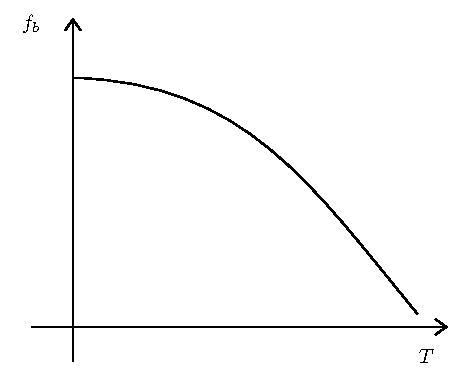
\includegraphics[width=0.5\textwidth]{../lessons/8_image/1.pdf}
\caption{\label{fig:8_1} Plot of the free energy \( f_b \) in function of the temperature \( T \). For \( T \rightarrow 0 \), the free energy becomes constant, while for \( T \rightarrow \infty  \) it goes linearly to zero.  }
\end{figure}
\end{itemize}

\subsubsection{The magnetization}
This can be obtained by differentiating the negative of the free energy with respect to the magnetic field \( H \) (or by using equation \eqref{eq:8_3}):
\begin{equation*}
  m = - \pdv{f_b}{H} = - \frac{1}{k_B T } \pdv{f_b}{h} = \pdv{}{h} \qty[  \log{\qty( \cosh(h)+\sqrt{\sinh^2(h)+e^{-4K}  } )} ]
\end{equation*}
The result is
\begin{equation}
  m =   \frac{\sinh h + \frac{ \sinh h \cosh h}{\sqrt{\sinh^2 h + e^{-4K} }} }{\cosh h + \sqrt{\sinh^2 h + e^{-4K} } } 
  = \frac{\sinh h  }{\sqrt{\sinh^2 h + e^{-4K} } }
  \label{eq:8_1}
\end{equation}
\begin{itemize}
\item Case: \( T>0 \) fixed, \( H \rightarrow 0 \Rightarrow h \rightarrow 0\).
\begin{subequations}
\begin{align*}
  \sinh h & \sim h \sim 0, \\ \cosh h &\sim 1
\end{align*}
\end{subequations}
In zero field \( h \rightarrow 0 \), we have \( m \rightarrow 0 \) for all \( T>0 \). It means that there is no spontaneous magnetization!
\end{itemize}


\subsubsection{The magnetic susceptibility}
\begin{equation}
  \chi_T  \equiv  \pdv{m}{H} = \frac{1}{k_B T} \pdv{m}{h}
\end{equation}
If we consider the case \( h \ll 1 \), it is convenient first expand the  \eqref{eq:8_1} for \( h \rightarrow 0 \) and take the derivative to get \( \chi _T \).

Since \( \sinh (h) \sim h+h^3 \) and \( \cosh (h) \sim 1 + h^2 \), we have
\begin{equation*}
  m \overset{h \ll 1}{\sim } \frac{h (1+e^{2K} )}{1+e^{-2K} }
\end{equation*}
If we now derive with respect to \emph{h}
\begin{equation*}
  \chi _T = \frac{1}{k_B T} \pdv{m}{h} \overset{h \ll 1}{\approx } \frac{1}{k_B T} \frac{(1+e^{2K} )}{(1+e^{-2K} )}
\end{equation*}
\begin{itemize}
\item Case: \( T \rightarrow \infty  \Rightarrow K \rightarrow 0\).
\begin{equation*}
  e^{2K} \simeq e^{-2K} \simeq 1
\end{equation*}
The \textit{Curie's Law} for paramagnetic systems is:
\begin{empheq}[box=\myyellowbox]{equation}
  \chi _T \sim \frac{1}{k_B T}
\end{empheq}
\item Case: \( T \rightarrow 0 \Rightarrow K \rightarrow \infty  \).
\begin{equation*}
  e^{-2K} \simeq 0
\end{equation*}
The \textit{Curie's Law} for paramagnetic systems is:
\begin{empheq}[box=\myyellowbox]{equation}
  \chi _T \sim \frac{1}{k_B T} e^{2K} \sim  \frac{1}{k_B T} e^{2J/k_B T}
\end{empheq}
\end{itemize}

\subsubsection{The correlation length}
\begin{equation}
  \xi ^{-1} = -\log{\qty(\frac{\lambda _-}{\lambda _+}) } = - \log{\qty[ \frac{\cosh h - \sqrt{\sinh^2 h + e^{-4K} } }{\cosh h + \sqrt{\sinh^2 h + e^{-4K} }}] }
\end{equation}
For \( h=0 \), we have \( \cosh h \rightarrow 1, \sinh h \rightarrow 0 \):
\begin{equation*}
  \xi ^{-1} = - \log{\qty[\frac{1- e^{-2K} }{1+ e^{-2K} }] } =  - \log{\qty[\frac{1 }{\coth K }] }
\end{equation*}
Therefore:
\begin{equation}
  \xi = \frac{1}{\log{ (\coth K )} }, \quad \text{for } h = 0
\end{equation}
\begin{itemize}
\item Case: \( T \rightarrow 0 \Rightarrow K \rightarrow \infty  \).
\begin{equation*}
  \coth K = \frac{e^{K} + e^{-K}  }{e^{K} - e^{-K}  } \overset{K \rightarrow \infty }{\simeq} 1 + 2 e^{-2K} + \dots \quad \overset{K \rightarrow \infty }{ \longrightarrow  } 1
\end{equation*}
It implies
\begin{equation*}
  \xi \overset{K \gg 1}{\sim } \frac{1}{\ln{(1+ 2 e^{-2K} )} } \sim \frac{e^{2K} }{2}
\end{equation*}
Hence,
\begin{equation}
  \xi \overset{T \rightarrow 0}{\sim } \frac{1}{2} e^{J/k_B T}
\end{equation}
It diverges exponentially \( \xi  \rightarrow \infty  \) as \( T \rightarrow 0 \).
\item Case: \( T \rightarrow \infty \Rightarrow K \rightarrow 0 \).
\begin{equation*}
  \coth K = \frac{e^{K} + e^{-K}  }{e^{K} - e^{-K}  } \overset{K \rightarrow 0 }{\simeq}
  \frac{1+K+\frac{K^2}{2}+1-K+\frac{K^2}{2}}{1+K+\frac{K^2}{2}-1+K-\frac{K^2}{2}}
  \sim \frac{2+2 \frac{K^2}{2}}{2K} \sim \frac{1+K^2}{K}
\end{equation*}
\begin{equation*}
  \xi ^{-1} = \log{(\coth K)} \overset{K \rightarrow 0}{\sim } \ln{\frac{1}{K}} + \ln{(1+K^2)} \sim + \infty
\end{equation*}
Therefore
\begin{equation*}
  \xi  \overset{K \rightarrow 0}{\longrightarrow} 0
\end{equation*}
More precisely,
\begin{equation}
  \xi \overset{K \rightarrow 0}{\sim } \frac{1}{\ln{(1/K)} + \ln{(1+K^2)}  } \overset{K \rightarrow 0}{\sim } - \frac{1}{\ln{K} }
\end{equation}

\end{itemize}







\section{Classical Heisenberg model for \emph{d=1} }

Now, let us suppose to study something different from the Ising model. Indeed, from a physicist's point of view the Ising model is highly simplified, the obvious objection being that the magnetic moment of a molecule is a vector pointing in any direction, not just up or down. One can build this property, obtaining the classical Heisenber model.
We do not anymore assume spin that can assume values as -1 or +1, but spin that can assume a continuous value. Unfortunately, this model has not been solved in even two dimensions \cite{9_lesson_4}.

Let us take a \( d=1 \) dimensional lattice.
In the classical Heisenberg model, the spins are unit length vectors \( \va{S}_i \), i.e. \( \va{S}_i \in \R^3 \), \( \abs{\va{S}_i}^2 = 1 \) (continuous values on the unit sphere). We have
\begin{equation*}
  \va{S}_i = ( S_i^x,S_i^y,S_i^z)
\end{equation*}
 with periodic boundary condition
\begin{equation*}
  \va{S}_{N+1} = \va{S}_1 
\end{equation*}
Assuming \( H=0 \), the model is defined through the following Hamiltonian:
\begin{equation}
  - \beta \mathcal{H} ( \{ \va{S} \}  ) = K \sum_{i=1}^{N} \va{S}_i \vdot \va{S}_{i+1}  \quad  (+ \sum_{i}^{} \va{h} \vdot \va{S}_i  )
\end{equation}
This model satisfies \( O(3) \) symmetry. In the transfer matrix formalism:
\begin{equation}
  Z_N (K) = \sum_{\{ \va{S} \}  }^{} e^{-\beta \mathcal{H}} = \sum_{\{ \va{S} \}  }^{} e^{K \sum_{i=1}^{N} \va{S}_i \vdot \va{S}_{i+1} } = \Tr(\mathbb{T}^N)
\end{equation}
where 
\begin{equation*}
\bra{\va{S}_i} \mathbb{T} \ket{\va{S}_{i+1}} = e^{K \va{S}_i \vdot \va{S}_{i+1}} 
\end{equation*}
Similarly to the Ising case, 
\begin{equation*}
  \mathbb{T} = \sum_{i}^{} \ket{t_i} \lambda _i \bra{t_i}
\end{equation*}
and
\begin{equation*}
  \mathbb{T}_D = \mathbb{P}^{-1} \mathbb{T}\mathbb{P}
\end{equation*}
The problem is computing the eigenvalues \( \lambda _i \) of \( \mathbb{T} \).

Formally, we should find
\begin{equation*}
  \exp [K \va{S}_1\vdot \va{S}_{2}] = \bra{\va{S}_1} \mathbb{T} \ket{\va{S}_2} = \sum_{i \in \text{\tiny eigenvalues}}^{} \lambda _i \braket{\va{S}_1}{t_i}  \braket{t_i}{\va{S}_2}
  = \sum_{i}^{} \lambda _i f_i ( \va{S}_1) f^* (\va{S}_2)
\end{equation*}

\begin{remark}
  We start by noticing that the term \( e^{K \va{S}_1 \cdot \va{S}_2}  \) is similar to the plane wave \(e^{i \va{q}\vdot \va{r}}  \), that in scattering problems is usually expanded in spherical coordinates. Plane wave can be expanded as a sum of spherical harmonics as
  \begin{equation*}
    e^{i \va{q}\vdot \va{r}} = 4 \pi \sum_{l=0}^{\infty } \sum_{m=-l}^{l} (i)^l j_l (qr) Y_{lm}^* (\vu{q}) Y_{lm} (\vu{r})
  \end{equation*}
  where
  \begin{equation*}
    j_l (qr) = - \frac{(i)^l}{2} \int_{0}^{\pi} \sin(\theta ) e^{i q r \cos(\theta ) } P_l (\cos(\theta ) ) \dd[]{\theta }
  \end{equation*}
  are the \emph{spherical Bessel functions}, while  the \( P_l (\cos(\theta ) ) \) are the \emph{Legendre polynomial} of order \emph{l}.
\end{remark}

From a formal comparison we have
  \begin{equation}
    \va{S}_1 \leftrightarrow \vu{S}_1, \qquad
      \begin{cases}
           i \va{q}\cdot \va{r} = iqr \\
           K \va{S}_1 \cdot \va{S}_2 = K \abs{\va{S}_1} \abs{\va{S}_2} = K
      \end{cases}
  \end{equation}
  multiplying by \( (-i) \)  we can write
  \begin{equation}
    qr = -iK \abs{\va{S}_1} \abs{\va{S}_2} = -iK
  \end{equation}
  In our case, we have
  \( \vu{q} = \va{S}_1, \vu{r} = \va{S}_2 \). Hence,
  \begin{equation}
    e^{K \va{S}_1 \cdot \va{S}_2} = 4 \pi  \sum_{l=0}^{\infty } \sum_{m=-l}^{l} (i)^l j_l (-iK) Y_{lm}^* (\va{S}_1) Y_{lm} (\va{S}_2) = \sum_{i}^{} \lambda _i f_i (\va{S}_1) f^* (\va{S}_2)
  \end{equation}
where
\begin{equation}
  \lambda _i = \lambda _{lm} (K) = 4 \pi (i)^l j_l (-iK)
\end{equation}
\begin{remark}
Note that \( \lambda _i \) does not depend on \emph{m}!
\end{remark}


If \( l=0 \), the largest eigenvalue is:
\begin{equation*}
  \lambda _+ = \lambda _0 (K) = 4 \pi j_0 (-iK) = 4 \pi \frac{\sinh K }{K}
\end{equation*}
and
\begin{equation*}
  \lambda _- = \lambda _1 (K) = 4 \pi i j_1 (-iK) = 4 \pi \qty[\frac{\cosh K }{K}-\frac{\sinh K }{K^2}]
\end{equation*}

\begin{exercise}{}{}
Given the largest eigenvalue \( \lambda _+ \),
\begin{equation*}
  \lambda _+ = 4 \pi \frac{\sinh K }{K}
\end{equation*}
find the bulk free energy density of the model and discuss its behaviour in the limits of low (\( T \rightarrow 0 \)) and high (\( T \rightarrow \infty  \)) temperatures.
\begin{solution}
The bulk free energy is 
\begin{equation*}
    f_b = -k_B T \log \lambda_+ = -k_B T \log \qty(  4 \pi \frac{\sinh K }{K} )
\end{equation*}
Remind that \( K \equiv \beta J \) and consider the limits
\begin{itemize}
    \item Case: \( T \rightarrow 0 \Rightarrow K \rightarrow \infty \).
    \begin{equation*}
       f_b = - \frac{J}{K} \log \qty(  4 \pi \frac{\sinh K }{K} )
        \overset{K \rightarrow \infty}{\sim}
        \frac{J}{K}   \log \qty(  \frac{K}{\sinh K} )
    \end{equation*}    
    Hence,
    \begin{equation*}
       f_b \overset{K \rightarrow \infty}{\sim} 0
    \end{equation*}      
    \item Case: \( T \rightarrow \infty \Rightarrow K \rightarrow 0 \).
    \begin{equation*}
        \sinh K \overset{K \rightarrow 0}{\sim} K
    \end{equation*}
    \begin{equation*}
        \Rightarrow f_b = - k_B T \log \qty(  4 \pi \frac{ \cancel{K} }{\cancel{K}} ) = - k_B T \log (4 \pi)
    \end{equation*}
    In this case the free energy \(f_b\) goes linearly with respect to the temperature.
\end{itemize}

\end{solution}
\end{exercise}


How can we violate the hypothesis of the Perron-Frobenius theorem hoping to find a phase transition also in a \( d=1 \) model?
 One of the hypothesis of the Perron-Frobenius theorem is the one in which \( A_{ij}>0  \) for all \(i,j \). Hence, one possibility is to build a model in which its transfer matrix has same \( A_{ij} \) that are equal to zero also for \( T \neq 0 \).

\end{document}
